\documentclass{article}
\usepackage{amsmath, amssymb}
\usepackage{pgfplots}
\usepackage[margin=1in]{geometry}
\usetikzlibrary{arrows.meta}

\begin{document}

\section{Plan for Class}
\begin{enumerate}
    \item Approximating invariant manifolds
    \item Diffeomorphisms/maps
    \item Stable manifold theorem for diffeomorphisms
    \item Transversal intersections 
    \item Hyperbolic .... automorphism
\end{enumerate}

\section{Points from last time}
We talked about the stable manifold theorem in order to make statements about the linearization $Df(x_0)=A$. Essentially, negative real part eigenvalues tells us that those subspaces (spanned by the eigenvectors) are stable and positive real part eigenvalues tells us that those subspaces (spanned by the eigenvectors) are unstable. For the matrix 
\[ A= \begin{bmatrix} -1 & 0 & 0 \\ 0 & -2 & 0 \\ 0 & 0 & 3  \end{bmatrix}\]
the eigenvectors for eigenvalues $-1,-2$ span $E^s$ and the eigenvectors for eigenvalue $3$ span $E^u$.

\section{Approximating invariant manifolds}
\subsection{Example}
Let's say we have the equation 
\begin{align*}
    \dot{x}&=x\\
    \dot{y}&=-y+x^2
\end{align*}
Our only fixed point is $(0,0)$. Linearization tells us 
\[ Df(x,y)= \begin{bmatrix} 1 & 0 \\ 2x & -1  \end{bmatrix}\]
Plugging in $(0,0)$, we get 
\[ Df(0,0)= \begin{bmatrix} 1 & 0 \\ 0 & -1  \end{bmatrix}\]
where we know what $E^s$ and $E^u$ are, but these only describe the behavior of the stable $W^s_{\text{loc}}$ and unstable manifolds $W^u_{\text{loc}}$ near the origin. Could we simply find these manifolds directly? Sometimes yes, but most cases no, but we can approximate them!

To approximate $W^u_{\text{loc}}$, we could write
\[ y=h(x)=a_0+a_1x+a_2x^2+a_3x^3+\cdots \]
where $a_0=0$ and $a_1=0$ via the stable manifold theorem (we know the eigenspace is tanget at the origin). Now we can write 
\[ h(x)= a_2x^2+a_3x^3+\text{ HOT}\]
We know that it's invariant via stable manifold theorem, so we can write 
\begin{gather*}
    \dot{y}=2a_2x\dot{x}+3a_3x^2\dot{x}+\text{ HOT}\\
    \implies -y+x^2=2a_2x\dot{x}+3a_3x^2\dot{x}+\text{ HOT}\\
    \implies -h(x)+x^2=2a_2x\dot{x}+3a_3x^2\dot{x}+\text{ HOT}\\
    \implies -\left(a_2x^2+a_3x^3\right)+x^2=2a_2x\dot{x}+3a_3x^2\dot{x}+O(x^4)
\end{gather*}
For $x^2$, our coefficient is 
\[a_2+1=2a^2\implies a_2=\frac{1}{3}\]
and for $x^3$, our coefficient is 
\[a_3=3 a_3\implies a_3=0\]
Hence, we can write 
\[ y=h(x)=\frac{x^2}{3}\]
and in this case, this is exact. To show this, we can write 
\[\dot{y}=-y+x^2=-\frac{x^2}{3}+x^2=\frac{2}{3}x^2\]
and 
\[ \frac{d}{dt}\left(\frac{x^2}{3}\right)=\frac{2}{3}x\dot{x}=\frac{2}{3}x^2 \]
and they agree.

\subsection{After class notes}
The example above will serve as a guide for how to do problem 3 in this weeks homework. Below, I take pains to show each step.

From linearization, we know 
\[ Df(0,0)= \begin{bmatrix} 1 & 0 \\ 0 & -1  \end{bmatrix}\]
and hence 
\[E^u=\operatorname{span}\left(\begin{bmatrix} 1 \\ 0 \end{bmatrix}\right) \]
which is equivalent to the equation $y=0+0x$ (the reason we are so explicit here will become clear).

We can imagine that our unstable, invariant manifold $W^u_{\text{loc}}$ can be represented as a line $y=h(x)$. Via the taylor series, we have 
\[ y=h(x)=a_0+a_1x+a_2x^2+a_3x^3+\cdots \]
where $a_0=0$ and $a_1=0$ via the stable manifold theorem. More explicitly, the stable manifold theorem tells us that $W^u_{\text{loc}}$ shares the same first derivative that we found via the linearization. Now we can write 
\[ h(x)= a_2x^2+a_3x^3+\text{ HOT}\]
This is where the fun begins! Our goal is to manipulate this expression $h(x)$ to reveal what $a_2$ and $a_3$ are. To make matters easier (in fact, achievable at all), we can use our time derivatives from the system to help us. To begin, lets take the derivative with respect to time to get 
\[ \dot{y}=2a_2x\dot{x}+3a_3x^2\dot{x}+\text{ HOT} \]
where we can plug in our expression $\dot{y}=-y+x^2$ to write 
\[ -y+x^2=2a_2x\dot{x}+3a_3x^2\dot{x}+\text{ HOT} \]
While this is weird, we have a previous expression for $y$ that we can make use of $y=h(x)$. Hence we have 
\[ -h(x)+x^2=2a_2x\dot{x}+3a_3x^2\dot{x}+\text{ HOT} \]
and then 
\[ -\left(a_2x^2+a_3x^3\right)+x^2=2a_2x\dot{x}+3a_3x^2\dot{x}+O(x^4) \]
Now we are going to make use of our expression for $\dot{x}=x$ to get 
\[ -\left(a_2x^2+a_3x^3\right)+x^2=2a_2x^2+3a_3x^3+O(x^4) \]
The pattern is clear. Let's group coefficients and solve
\[ (1-a_2)x^2-a_3x^3=2a_2x^2+3a_3x^3+O(x^4) \]
For $x^2$, our coefficient is 
\[a_2+1=2a^2\implies a_2=\frac{1}{3}\]
and for $x^3$, our coefficient is 
\[-a_3=3 a_3\implies a_3=0\]
Hence, we can write 
\[ y=h(x)=\frac{x^2}{3}\]

\section{Diffeomorphisms/maps}
Let's remind ourselves what maps. A flow is $\dot{x}=f(x)$ and a map is $x_{t+1}=F(x_t)$. For flows, we have a version of a map
\[\phi_t : x(0)\mapsto x(t)\] 
where $(\phi_t)^{-1}=\phi_{-t}$. For maps, we have something similar to $\phi_t$ written as $F=\phi_{\Delta t}$.

If $F$ comes from a flow ($F=\phi_{\Delta t}$) then $F$ is invertible, and usually differentiable (with differetiable inverse): i.e. $F$ is a diffeomorphism.

\subsection{Let's say more about maps}
We can work with non-invertible maps too.
\subsubsection{Example}
\[ x_{t+1}=\mu x_t (1-x_t)=F(x_t) \]
where fixed points occur at $F(x_0)=x_0$. To visualize the plot, for $\mu \geq 0$ we have a parabola with roots $x=0$ and $x>0$.

\begin{figure}[h]
\centering
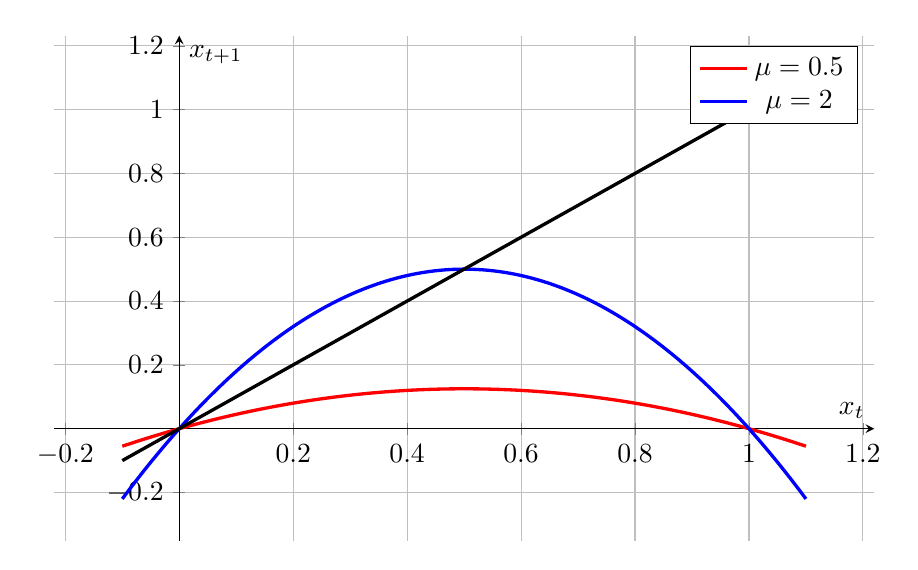
\begin{tikzpicture}
\begin{axis}[
  xlabel={$x_t$},
  ylabel={$x_{t+1}$},
  grid=major,
  width=12cm,
  height=8cm,
  domain=-0.1:1.1,
  samples=200,
  axis lines=middle,
  enlargelimits=true,
]
\addplot[red, very thick] {0.5*x*(1-x)};
\addlegendentry{$\mu=0.5$}
\addplot[blue, very thick] {2*x*(1-x)};
\addlegendentry{$\mu=2$}
\addplot[black, very thick] {x};

\end{axis}
\end{tikzpicture}
\caption{Logistic map for different values of $\mu$}
\end{figure}
As we can see in the plot, for $\mu>1$, we get a fixed point along $y=x$. 

There's a lot of cobweb diagrams being draw to demonstrate the stability for maps graphically. These are rather standard, so we can include these later. In general, the statements are 
\begin{itemize}
    \item $0<f'(x)<1$ is stable 
    \item $f'(x)>$ is unstable 
    \item $-1<f'(x)<0$ is stable 
    \item $f'(x)<-1$ is unstable 
\end{itemize}
Therefore, we are stable if $\left|f'(x)\right|<1$ and unstable if $\left|f'(x)\right|>1$

\subsubsection{What about higher dimensions?}
Let's say that $x\in\mathbb{R}^n$ and 
\[ x(t+1)=F(x(t)) \]
Again, we have equilibrium points at $x_0$ for $F(x_0)=x_0$. We can do something akin to linearization by writing $x(t)=x_0+\xi (t)$ and 
\[ x_0+\xi (t+1)=x(t+1)=F(x_0+\xi)=F(x_0)+DF(x_0)\xi + O(\xi^2) \]
where simplifing gets us 
\[ \xi(t+1)=DF(x_0)\cdot \xi(t) + \text{ HOT} \]
One again, we have $A=DF(x_0)$ and we can look at the eigenvalues of $A$. For the following eigenvalues, we can state 
\begin{itemize}
    \item $|\lambda |>1$ is an unstable eigenvalue 
    \item $|\lambda |<1$ is a stable eigenvalue
\end{itemize}
Our linearization looks something like 
\begin{align*}
    \xi(0)&=v\qquad\text{where $v$ is an eigenvector}\\
    \xi(1)&=Av=\lambda v\\
    \xi(2)&=A\xi(1)=A(\lambda v)=\lambda^2v
\end{align*}
Hence, we can write 
\[\xi(t)=\lambda^t v \] 
and can state 
\begin{itemize}
    \item If $|\lambda|>1$, then $|\lambda^t|\to\infty$ as $t\to\infty$
    \item If $|\lambda|<1$, then $|\lambda^t|\to 0$
    \item If $|\lambda|=1$, then it's inconclusive
\end{itemize}

\subsubsection{Are there things that are different with maps than flows?}
As an example, let's say 
\[ A= \begin{bmatrix} \lambda_1 & 0 \\ 0 & \lambda_2 \end{bmatrix}\]
\begin{itemize}
    \item For $\lambda_2>\lambda_1$, we get smooth like trajectories to the origin, just as in flows.
    \item For $\lambda_1<0<\lambda_2$, we get zig-zag like trajectories to the origin, where $z_1$ is fliping across the $z_2$ axis at each step.
    \item For $\lambda_2<\lambda_1<0$, we get zig-zag like trajectories to the origin, where $z_1$ and $z_2$ are constantly flipping across the axes.
\end{itemize}
Said another way, for $\det A>0$ we have \textit{orientation preserving} trajectories. For $\det A <0$ we have \textit{orientation reversing} trajectories.

\subsection{Diffeomorphism}
Now we'll assum $F$ is a diffeomorphism ($C^1$ with $C^1$ inverse).

Definition: $p$ is a fixed point of $F$ ($F(p)=p$). If no eigenvalue of $DF(p)$ has unit modulus (i.e. on unit circle) then $p$ is hyperbolic.

Stable manifold theorem: For diffeomorphisms, we can define $W^s_{\text{loc}}$ and $W^u_{\text{loc}}$ exactly as in ODE case. Let $G:\mathbb{R}^n\to\mathbb{R}^n$ be a $C^1$ diffeomorphism with a hyperbolic fixed point $p_0$. The there exists a local stable and unstable manifolds $W^{u,s}_{\text{loc}}(p_0)$ tangent at $p$ to stable/unstable eigenspaces $E^{s,u}$ respectively. With $W^{u,s}_{\text{loc}}(p_0)$ being as smooth as $G$.

Also take a peak at Hartman-Grobman theorem for maps (theorem 1.4.1).

\section{Transversal intersections}
We can extend $W^{u,s}_{\text{loc}}(p)$ to global stable and unstable manifolds $W^{u,s}(p)$ by starting with a small piece of $W^{u,s}_{\text{loc}}(p)$ and iterating ther points forward and backward. But $W^{s}$ cannot intersect itself, and $W^{u}$ cannot intersect itself, but can $W^{s}$ intersect $W^{u}$? Yes! This happens with homoclinic orbits.

I don't know how we got here, but the definition of a transversal intersection is 
\[ T_pM_1\bigcup T_pM_2=\mathbb{R}^n \]
Which means that two manifolds ``transversally intersect'' if they intersect in a non parallel fashion. Like, two perpendicular lines intersect transversally, but two parallel lines don't.

\end{document}